%# -*- coding: utf-8-unix -*-
% !TEX program = xelatex
% !TEX root = ../thesis.tex
% !TEX encoding = UTF-8 Unicode
\chapter{传感器}
\label{chap:sensor}
\section{全球定位系统}
全球定位系统(Global Positioning System,GPS)是一种以空中卫星为基础的高精度无线电导航的定位系统,
它在全球任何地方以及近地空间都能够提供准确的地理位置、刚体速度及精确的时间信息。
对于室外定位,一般采用GPS或者北斗定位系统。


\subsection{GPS定位定向天线 Hemisphere V102}
Hemisphere V102提供定向、定位、起伏、横滚和俯仰信息,可利用SBAS差分GPS定位,水平精度为
0.5 m; 侧向精度为$0.75^{\circ}$, 俯仰/横滚精度为$1.5^{\circ}$。
使用时推荐采样频率10 Hz, 波特率为115200。
在串口助手里面(cutecom或者sscom)可输入指令(见表\ref{tab:V102command}),
修改V102输出的内容。由于V102不支持北斗功能,与北斗相关的命令是无效的。
每次设置完GPS之后,记得\$JSAVE保存配置


% Table generated by Excel2LaTeX from sheet 'Sheet1'
\begin{table}[htbp]
  \centering
  \caption{Hemisphere V102常用指令}
    \begin{tabular}{p{11.54em}p{19.96em}}
    \toprule
    命令    & 功能 \\
    \midrule
    \$JSHOW & 查询V102的设置 \\
    \$JDIFF & 查询当前差分模式 \\
    \$JDIFF, INCLUDE, SBAS & 设置SBAS参与差分定位 \\
    \$JBAUD, X & 设置当前串口波特率为X, 推荐X=115200 \\
    \$JASC, GPGGA, X & 设置NMEA GPGGA消息的输出频率为 X Hz; 若X=0, 不输出GPGGA的数据;推荐X=10 \\
    \$JASC, GPGSV, X & 设置NMEA GPGSV消息的输出频率为 X Hz \\
    \$JASC, GPHDT, X & 设置NMEA GPHDT消息的输出频率为 X Hz \\
    \$JASC, GPHPR, X & 设置NMEA GPGSV消息的输出频率为 X Hz \\
    \$JASC,GPROT,X & 首向速度(deg/min) \\
    \$JASC, PSAT,ATTSTAT, X & 打开副天线卫星信息,同时包含基线长等信息 \\
    \$JASC, PVCT, X & 输出主副天线的东向,北向,及天向的差值 \\
    \$JATT,GYROAID,YES & 打开陀螺 \\
    \$JATT,GYROAID & 查询陀螺当前状态 \\
    \$JATT,TILTAID,YES & 打开倾斜传感器 \\
    \$JATT,TILTAID & 查询当前倾斜传感器的状态 \\
    \bottomrule
    \end{tabular}%
  \label{tab:V102command}%
\end{table}%

% Table generated by Excel2LaTeX from sheet 'Sheet1'
\begin{table}[htbp]
  \centering
  \caption{防水接头接线方法}
    \begin{tabular}{lp{3.25em}lp{19.25em}}
    \toprule
    \multicolumn{1}{p{3.125em}}{Pin} & 颜色    & \multicolumn{1}{p{3.29em}}{Pin(*)} & 功能 \\
    \midrule
    1     & 白     & 1     & Port C, RS-232 female DB9 pin 2, device out \\
    2     & 绿     & 3     & Port C, RS-232 female DB9 pin 3, device in \\
    5     & 红     & 5     & Power input \\
    7     & 黄     & 2     & Signal Ground \\
    8     & 棕     & 7     & Port A, RS-232 female DB9 pin 3, device in \\
    9     & 蓝     & 6     & Port A, RS-232 female DB9 pin 2, device out \\
    10    & 黑     & 4     & Power Ground \\
    11    & Drain  & 8     & CH\_GND \\
    \bottomrule
    \end{tabular}%
    \begin{tablenotes}
        \footnotesize
        \item[*] 注: Pin指的是V102上的12芯防水接头上的数字,Pin(*)指的是控制盒上
        8芯防水接头上的数字;在控制盒中,Signal Ground一分为二,黄色和灰色线共用。
    \end{tablenotes}
  \label{tab:pluginconnect}%
\end{table}%


\subsection{墨卡托投影}
墨卡托投影,是正轴等角圆柱投影。由荷兰地图学家墨卡托(G.Mercator)于1569年创立。
假想一个与地轴方向一致的圆柱切或割于地球,按等角条件,将经纬网投影到圆柱面上,
将圆柱面展为平面后,即得本投影。墨卡托投影在切圆柱投影与割圆柱投影中,
最早也是最常用的是切圆柱投影。
首先,我们来了解一些常用的导航坐标系
\begin{itemize}
  \item 地理坐标系(Geographic coordinates)地理坐标系一般是指由经度、纬度和相对高度组成
  的坐标系,能够标示地球上的任何一个位置。
  \item 通用横轴墨卡托投影(Universal Transverse Mercator,简称UTM) \cite{hager1989universal} 是一种国际标准化的地图投影法。它使用笛卡尔坐标系,
  标记南纬$80^{\circ}$至北纬$84^{\circ}$之间的所有位置。本坐标系采用WGS84系统作为坐标基础。
  \item 通用极立体坐标系(Universal polar stereographic coordinate system,简称UPS)作为
  UTM的补充,标记南纬$80^{\circ}$以南和北纬$84^{\circ}$以北的所有位置,以及与UTM有$0.5^{\circ}$的重叠。
\end{itemize}

值得注意的是,跨越UTM区域的时候会出现坐标不连续的问题。这里我们在UTM区域之间
引入100公里(100 km)的重叠区(如图\ref{fig:utmoverlap}),从而解决坐标不连续的问题。同时,
在路径规划算法中,用户输入的坐标点需要经过计算,确保Waypoints或者DP setpoint在同一个
UTM区域且不超过100km。

\begin{figure}[!htp]
  \centering
  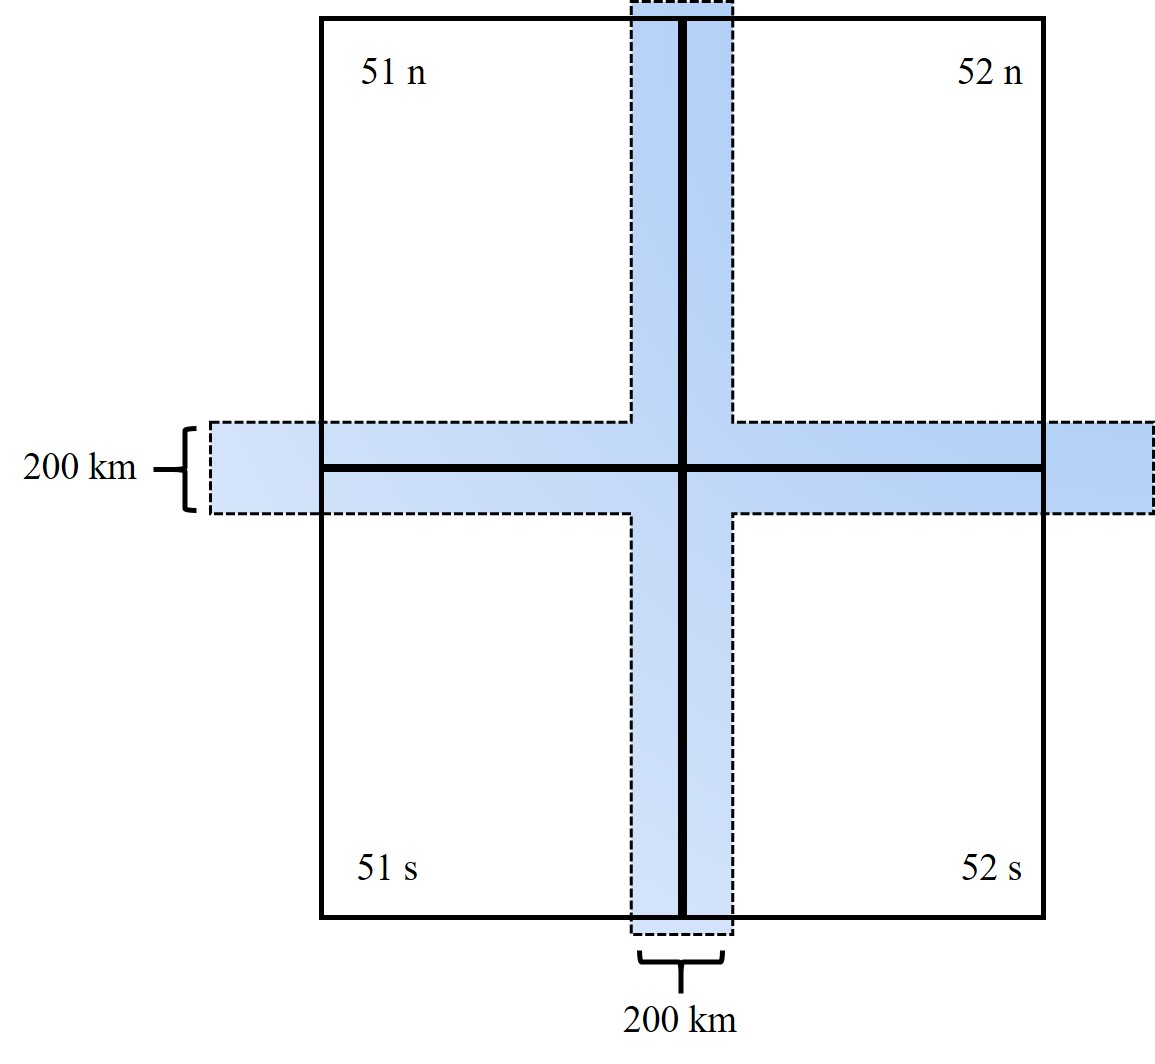
\includegraphics[width=10cm]{chapter_sensor/utmoverlap.jpg}
  \bicaption[UTM区域的重叠]
    {UTM区域的重叠}
    {The overlap between UTM zones}
  \label{fig:utmoverlap}
\end{figure}


\section{惯性测量单元}
惯性测量单元(Inertial measurement unit,简称IMU是测量物体三轴姿态角(或角速率)以及加速度的装置。

\section{航海雷达}
\section{红外热像仪}
\section{风速风向仪}
